\section{Iteration \#1 -- Evaluation Framework, Baselines and the Pyramid Tree}

The first iteration was chosen to be two weeks long, instead of just one. This was to accommodate the extra work that would need to be done initially to lay the foundations that would be used to implement and evaluate the implementations. The objectives for this iteration were:
\begin{itemize}
	\item Design and implement a standard framework for evaluating index structures in C++
	\item Implement evaluation baselines (Sequential Scan and Octree)
	\item Incorporate the School's implementation of the Pyramid Tree into framework
	\item Analyse performance of two baselines and the Pyramid Tree, evaluating their performance
\end{itemize}

TODO: mention original plan of implementing the Splay quadtree???

\subsection{Evaluation Framework}

The evaluation framework implemented in the first week of this iteration was created to define the standard data used across the index structures, provide a way of loading point datasets and operation lists and feeding them to index structures. There are three core modules of the framework:

\begin{wrapfigure}[12]{r}{0.5\textwidth}
	\vspace{-40pt}
	\begin{center}
		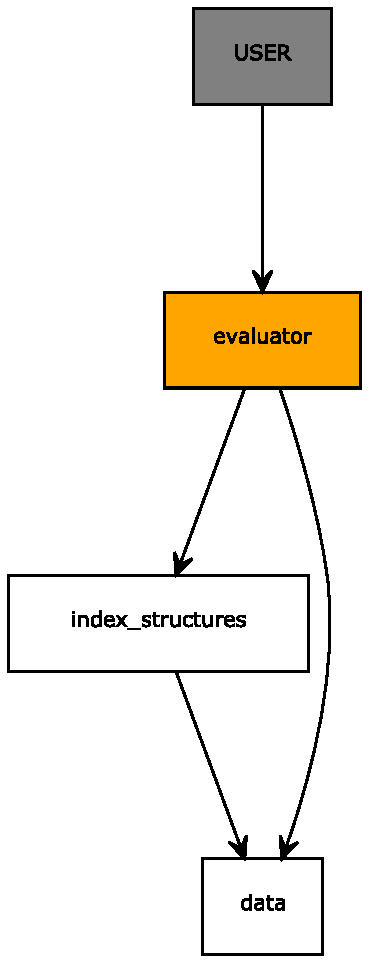
\includegraphics[scale=0.4]{figures/evaluation_framework.pdf}
	\end{center}
	\vspace{-20pt}
	\caption{Modules of Evaluation Framework}
	\label{fig:evaluation-framework}
\end{wrapfigure}

\begin{itemize}
	\item \texttt{data} -- library that contains standard data types used throughout framework and index structures, as well as dataset and test operation generators/loaders
	\item \texttt{index\_structure} -- library that contains all the index structures implemented throughout the project
	\item \texttt{evaluator} -- executable program that takes the index structures, operation lists and other options from the command line and runs a set of automated performance tests that produces timings and profiling (CPU and heap) information
\end{itemize}

The \texttt{evaluator} executable facilitates fast evaluation by allowing multiple index structures to be tested at once, using multiple tests operation lists (as described in Chapter \ref{chap:evaluation-outline}) at once. It stores timings in text files which are fed into bash and Gnuplot scripts to generate plots, which can be understood and incorporated into the report with ease. Figure \ref{fig:evaluation-framework} illustrates the modules of the framework, showing how user performing the performance evaluation only directly interacts with the \texttt{evaluator} executable.

The framework was created because performance analysis would be done very frequently, multiple times per iteration. Manually timing and profiling the code each time is time-consuming and error-prone. Putting more effort initially into creating a system that allows large sets of operations and index structures to be tested at once may save a significant amount of time , especially as many of these performance test are long and must be run multiple times to get averages.

Every index structure defined in the \texttt{index\_structures} module implement the \texttt{IndexStructure} interface, which has the following methods:
\begin{itemize}
	\item \texttt{loadPoints} -- bulk load a collection of points into structure
	\item \texttt{clear} -- remove all points from structure
	\item \texttt{insert} -- insert point into structure (if it's not already stored, see assumption (4) in Section \ref{sec:core-assumptions})
	\item \texttt{remove} -- remove point from structure
	\item \texttt{update} -- modify value of a specific point stored in the structure
	\item \texttt{pointExists} -- equivalent to a point query
\end{itemize}

\subsection{Baseline Implementations}
 
Sequential scan was implemented using the C++ container \texttt{std::vector}, a dynamically resizeable array. Points insertion is $O(1)$ as they are added to the end of the vector and deleting points results in a standard array deletion, making it an $O(n)$ operation. Point queries are performed in $O(n)$ time, as the query iterates through the array sequentially until the given point is found or the end of the array is reached.

The octree variant implemented as a baseline is a bucket PR octree. This means the structure partitions the underlying data space into uniformly sized boxes, without using the points as pivots (unlike point quadtrees or kd-trees). It is a bucket octree because \textit{multiple} points can be stored in a single leaf node. The octree dynamically decomposes and composes spatial regions based on its current contents. When the number of points in a leaf node exceeds a certain number, say $M$, then the region represented by the leaf is sub-divided, creating $2^d$ children. The $M + 1$ points are then scattered across the children. Therefore, regions of space that contain more points are decomposed more and sparse regions of space have less granularity, meaning less nodes and memory overhead.

When a point is deleted from a leaf, the contents of the leaf and all of its siblings are checked. If all of these nodes are empty, they are removed and the sub-regions are combined into the original region again. If the now collapsed parent and all of its siblings are empty, then they are collapsed into their parent. This is repeatedly recursively until a parent is reached whose children contain at least one point.

\subsection{Pyramid Tree}

As described in Section \ref{sec:pyramid-tree}, the Pyramid tree reduces multi-dimensional points to one dimension, which can then be used in a one-dimensional index structure. The School of Computing have an existing implementation of the Pyramid tree, written by Zhao Geng\footnote{Z.Geng@leeds.ac.uk}. While Berchtold et al. in \cite{pyramid-tree} used a B${}^{+}$-tree as the underlying 1D structure, this implementation uses a hash map (specifically \texttt{boost::unordered\_map}). All the points are stored in a single \texttt{std::vector}. Each point is hashed to an integer representation which acts as the key to a bucket stored in the hash map. A bucket is a \texttt{std::vector} which contains indices to points in the large point array.
 
Simple optimisations were initially made to the original implementation. The original implementation passed many heap allocated structures by-value, resulting in excessive copies and more time being spent allocating memory and copying data. These copies were not necessary and were removed where possible by passing the data by-reference.

The original Pyramid tree implementation did not provide \texttt{delete} and \texttt{update} operations. Therefore, a \texttt{delete} procedure was added to the implementation. To delete a point $p$, the point is first hashed and the bucket containing the point is found. The index pointing to $p$ in the bucket is removed from the bucket, but the actual point itself is not removed the point array. In other words, the memory is never released until the whole structure is deleted. This makes the structure useful for batch computation because it can be discarded straight after a task, releasing all allocated memory then. However, if the structure is used as part of a long-running process then this is not suitable because there is the potential to run out of memory. This will be referred to as the \textbf{Batch Index Pyramid Tree} for the rest of this document.

Therefore, a variant of this structure was implemented, which shall be referred to as the \textbf{Defragmented Index Pyramid Tree}. When a point's index is deleted from a bucket, the element at the index is marked for deletion from the array at a later time (by adding the index of the point to another \texttt{std::vector}). If the number of marked elements exceeds a certain number $R$, then the $R + 1$ marked elements are erased from the vector (i.e. memory is released). The indices in each bucket are then updated to point to the correct element in the modified array. Even though \texttt{delete} is normally a constant time operation, the worst case is $O(n^2)$ because of this defragmentation procedure.

\subsection{Compiler Optimisation}

GCC\footnote{GCC, the GNU Compiler Collection -- \url{http://gcc.gnu.org/}} was the C++ compiler used throughout development and analysis. GCC provides options to automatically modify the source code to make it more efficient on the target platform. There are multiple levels of optimisations, specifying using command line flags, going from 0 (\texttt{-O0} flag, no optimisation) to 3 (\texttt{-O3} flag, maximum optimisation). The default optimisation level is 0. In order to make the structures as fast as possible, level 3 optimisation was used to compile the structures. Table \ref{tab:compiler-optimisation} shows the average execution times for the three operations for each structure, using a 10D random uniformly distributed dataset with 10,000 points. The potential speed gains are huge. For example, the octree's point queries are approximately $6.5$ times faster, just by enabling level 3 optimisation.

\begin{table}
	\centering
	\begin{tabular}{|l|l|l|l|}
		\hline
		\textbf{Structure} & \textbf{Operation} & \texttt{-O0} & \texttt{-O3} \\
		\hline
		\multirow{ 4}{*}{\textbf{Sequential Scan}} & \textbf{Insert} & 1.33509 & 0.111372 \\
		 & \textbf{Delete} & 5.29548 & 0.623759 \\
		 & \textbf{Point Query} & 1.33468 & 0.111909 \\
		\hline
		\multirow{ 4}{*}{\textbf{Octree}} & \textbf{Insert} & 1.23108 & 0.243256 \\
		 & \textbf{Delete} & 0.73156 & 0.13589 \\
		 & \textbf{Point Query} & 0.559736 & 0.0860926 \\
		\hline
		\multirow{ 4}{*}{\textbf{Batch Index Pyramid Tree}} & \textbf{Insert} & 0.0240852 & 0.00549841 \\
		 & \textbf{Delete} & 0.0108411  & 0.0023433 \\
		 & \textbf{Point Query} & 0.0103358 & 0.00242341 \\
		\hline
		\multirow{ 4}{*}{\textbf{Defragmented Index Pyramid Tree}} & \textbf{Insert} & 0.0236123 & 0.00558329 \\
		 & \textbf{Delete} & 13.3113 & 1.49306 \\
		 & \textbf{Point Query} & 0.0103173 & 0.00235689 \\
		\hline
	\end{tabular}
	\caption{Execution Time (in Seconds) of Structure Operations With and Without Compiler Optimisations (10D Randomly Uniform  Dataset, 10,000 points used)}
	\label{tab:compiler-optimisation}
\end{table}

While the potential performance boost can be high, there are some downsides to compiler optimisation. Using full optimisaiton can increase the size of the program binaries and it makes the program harder to debug, because the code is restructred and managed, making it difficult to get a method call trace \cite{gcc}. This also makes applications harder to profile. One could profile an application using no optimisation to avoid this issue, but there is no guarantee that functions/methods which are bottlenecks in the non-optimised binary are still bottlenecks in the fully optimised binary. Therefore, optimising the code to remove particular bottlenecks in the non-optimised version may have little, if no, impact on the fully optimised binary (which ptoentially still performs faster).

To summarise, full compiler optimisation will be used during performance analysis of the structures as the speed gains can be huge. Despite CPU profiling potentially being harder to understand and less useful on fully optimised binaries, this shall still be done over profiling the non-optimised binary because of the aforementioned reasons.

\subsection{Performance Timings}

For this analysis, the three synthetic datasets described in Section \ref{sec:datasets} were used, each having $10000$ points and varying dimensions. Each of the three operations -- \texttt{insert}, point queries and \texttt{delete}, are tested by inserting all points in the structure, querying all points and then deleting all points from the dataset respectively. Timestep 100 of the astrophysics turbulence simulation was also used at an eighth of the resolution, producing a uniformly sampled $75 \times 31 \times 31$ grid with $72075$ points, with two different operation lists. The first list inserts all points in the sampeld ataset, queries them and deletes them. The secnod is a sequence of random operations that use the points from the sampled dataset. The structures being analysed in this iteration are sequential scan, octree and the index pyramid trees (batch and defragmented). A value of 3000 was chosen for $R$, meaning the Defagmented Index Pyramid Tree defragments when 3001 elements have been marked for deletion.

Table \ref{tab:perf1-randuniform} shows the \textit{total} runtime of \texttt{insert}, \texttt{delete} and point query operations for uniformly randomly generated points.Multiple datasets, with different dimensions, were used to observe how the structure's performance behaves as the dimensionality is increased.  When \`-" is shown instead of the number of seconds, it means that the performance test could not finish due to the machine running out of memory. The execution times for skewed and clustered data was almost identical to the uniformly random datasets; for the sake of brevity, the tables and plots for these datasets have been placed in Appendix \ref{chap:supp-material}. Table \ref{tab:perf1-astrophysics} shows the total runtime of the two astrophysics dataset operation lists.

In addition to testing performance with respect to dimensionality, the structures have been tested against data of varying size. A uniformly randomly generated dataset with 1,000,000 points has been created. The performance of the three operations has been timed for different sized datasets, sampled from the 1,000,000 point dataset. Again, the three operations are timed using the insert-query-delete sequences of operations. The times are displayed in Table \ref{tab:perf1-sizevary} and Figures \ref{fig:perf-sizevary-insert}, \ref{fig:perf-sizevary-delete} and \ref{fig:perf-sizevary-query}. Since the number of operations \textit{varies} for each dataset, unlike the previous two tests, the times given in the table and plots is the \textit{average} operation time, not the \textit{total}, so a per-operation comparison can be made.

\begin{landscape}

	\begin{table}
		\centering
		\begin{tabular}{|p{2cm}|l|l|l|l|l|l|l|l|l|l|l|}
			\hline
			\textbf{Structure} & \textbf{Operation} & \textbf{1D} & \textbf{2D} & \textbf{3D} & \textbf{5D} & \textbf{8D} & \textbf{10D} & \textbf{30D} & \textbf{50D} & \textbf{100D} & \textbf{200D} \\
			\hline
			\multirow{ 4}{*}{\textbf{Sequential Scan}} & \textbf{Insert} & 0.083928 & 0.0856602 & 0.0858041 & 0.0970701 & 0.0960585 & 0.11025 & 0.13113 & 0.135196 & 0.142939 & 0.142896 \\ & \textbf{Delete} & 0.46229 & 0.577141 & 0.696159 & 0.688754 & 0.634093 & 0.623097 & 0.71913 & 0.882381 & 1.50442 & 3.29082 \\ & \textbf{Point Query} & 0.0834135 & 0.0842911 & 0.0849031 & 0.095202 & 0.0950359 & 0.110287 & 0.130051 & 0.134541 & 0.140541 & 0.142191 \\
			\hline
			\multirow{ 4}{*}{\textbf{Octree}} & \textbf{Insert} & 0.00342762 & 0.0031842 & 0.00361466 & 0.0102806 & 0.0368217 & 0.241889 & - & - & - & - \\ & \textbf{Delete} & 0.00299168 & 0.00256801 & 0.00275838 & 0.00641203 & 0.0259533 & 0.132478 & - & - & - & - \\ & \textbf{Point Query} & 0.00244093 & 0.00213456 & 0.00217879 & 0.00487924 & 0.0229579 & 0.086069 & - & - & - & - \\
			\hline
			\multirow{ 4}{*}{\textbf{Batch Index Pyramid Tree}} & \textbf{Insert} & 0.00182509 & 0.00201285 & 0.00209451 & 0.00268757 & 0.0040772 & 0.00534821 & 0.0345241 & 0.0927804 & 0.365613 & 1.45883 \\ & \textbf{Delete} & 0.000421524 & 0.000508428 & 0.000604391 & 0.000930548 & 0.00166643 & 0.0023284 & 0.0171595 & 0.0467448 & 0.183702 & 0.728678 \\ & \textbf{Point Query} & 0.000406027 & 0.00050652 & 0.000588536 & 0.00090754 & 0.00173366 & 0.00235772 & 0.0171422 & 0.046788 & 0.183745 & 0.729757 \\
			\hline
			\multirow{ 4}{*}{\textbf{Defragmented Index Pyramid Tree}} & \textbf{Insert} & 0.00182939 & 0.0019474 & 0.0020951 & 0.00262773 & 0.00407147 & 0.00530696 & 0.0345504 & 0.0927966 & 0.36549 & 1.45541 \\ & \textbf{Delete} & 1.31443 & 1.40514 & 1.48344 & 1.49642 & 1.43011 & 1.48568 & 1.52637 & 1.66116 & 2.21606 & 3.94223 \\ & \textbf{Point Query} & 0.00040555 & 0.000497341 & 0.000604749 & 0.000905514 & 0.00168335 & 0.00233459 & 0.0172749 & 0.046602 & 0.183578 & 0.729738 \\
			\hline
		\end{tabular}
		\caption{Total Execution Time (in Seconds) of 10,0000 Structure Operations for Uniformly Random Points}
		\label{tab:perf1-randuniform}
	\end{table}

	\begin{table}
		\centering
		\begin{tabular}{|p{2cm}|l|l|l|l|l|l|l|l|l|}
			\hline
			\textbf{Structure} & \textbf{Operation} & $n = 10$ & $n = 100$ & $n = 1000$ & $n = 5000$ & $n = 10000$ & $n = 50000$ & $n = 100000$ & $n = 500000$ \\
			\hline
			\multirow{ 4}{*}{\textbf{Sequential Scan}} & \textbf{Insert} & 0 & 0 & 0 & 0 & 0 & 0 & 0 & 0 \\
			 & \textbf{Delete} & 0 & 0 & 0 & 0 & 0 & 0 & 0 & 0 \\ & \textbf{Point Query} & 0.0834135 & 0.0842911 & 0.0849031 & 0.095202 & 0.0950359 & 0.110287 & 0 & 0 \\
			\hline
			\multirow{ 4}{*}{\textbf{Batch Index Pyramid Tree}} & \textbf{Insert} & 0.00182509 & 0.00201285 & 0.00209451 & 0.00268757 & 0.0040772 & 0.00534821 & 0.0345241 & 0.0927804 \\ & \textbf{Delete} & 0.000421524 & 0.000508428 & 0.000604391 & 0.000930548 & 0.00166643 & 0.0023284 & 0.0171595 & 0.0467448 \\ & \textbf{Point Query} & 0.000406027 & 0.00050652 & 0.000588536 & 0.00090754 & 0.00173366 & 0.00235772 & 0.0171422 & 0.046788 \\
			\hline
			\multirow{ 4}{*}{\textbf{Defragmented Index Pyramid Tree}} & \textbf{Insert} & 0.00182939 & 0.0019474 & 0.0020951 & 0.00262773 & 0.00407147 & 0.00530696 & 0.0345504 & 0.0927966 \\ & \textbf{Delete} & 1.31443 & 1.40514 & 1.48344 & 1.49642 & 1.43011 & 1.48568 & 1.52637 & 1.66116 \\ & \textbf{Point Query} & 0.00040555 & 0.000497341 & 0.000604749 & 0.000905514 & 0.00168335 & 0.00233459 & 0.0172749 & 0.046602 \\
			\hline
		\end{tabular}
		\caption{Average Execution Time (in Seconds) of $n$ Structure Operations for $n$ Uniformly Random Points}
		\label{tab:perf1-sizevary}
	\end{table}


	\begin{table}
		\centering
		\begin{tabular}{|r|l|l|}
			\hline
			\textbf{Structure} & \textbf{InsertAll-QueryAll-DeleteAll} & \textbf{10,000 Random Operations} \\
			\hline
			\textbf{Sequential Scan} & 17.6743 & 8.92193 \\
			\textbf{Octree} & - & - \\
			\textbf{Batch Index Pyramid Tree} & 2.72248 & 3.66369 \\
			\textbf{Defragmented Index Pyramid Tree} & 12.6136 & 6.22732 \\
			\hline
		\end{tabular}
		\caption{Total Execution Time (in Seconds) for Sampled Astrophysics Dataset}
		\label{tab:perf1-astrophysics}
	\end{table}	

\end{landscape}

\begin{figure}
	\centering
	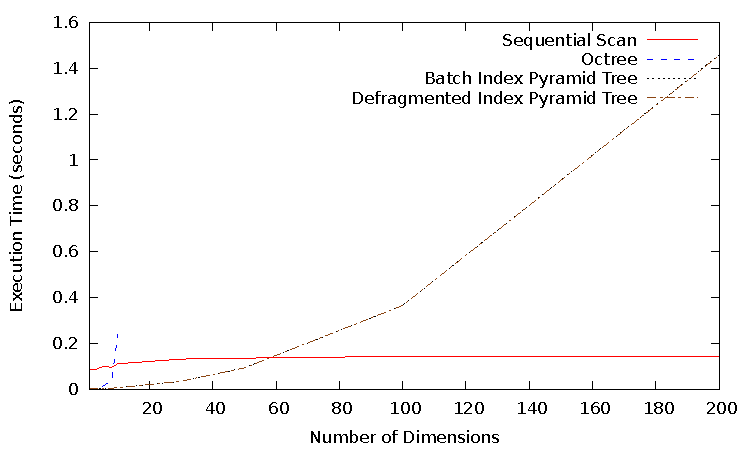
\includegraphics[scale=0.8]{figures/performance_analysis/iteration_1/all_insert_randuniform.pdf}
	\caption{\texttt{insert} Performance on Randomly Generated Uniformly Distributed Datasets}
	\label{fig:perf-1-allinsert-d}
\end{figure}

\begin{figure}
	\centering
	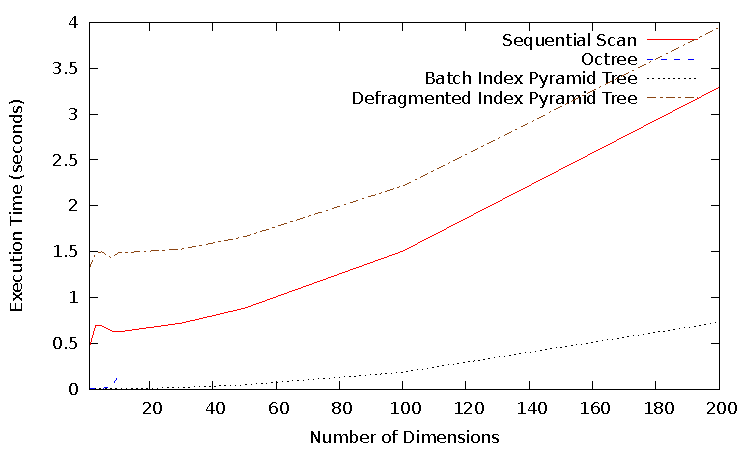
\includegraphics[scale=0.8]{figures/performance_analysis/iteration_1/all_delete_randuniform.pdf}
	\caption{\texttt{delete} Performance on Randomly Generated Uniformly Distributed Datasets}
	\label{fig:perf-1-alldelete-d}
\end{figure}

\begin{figure}
	\centering
	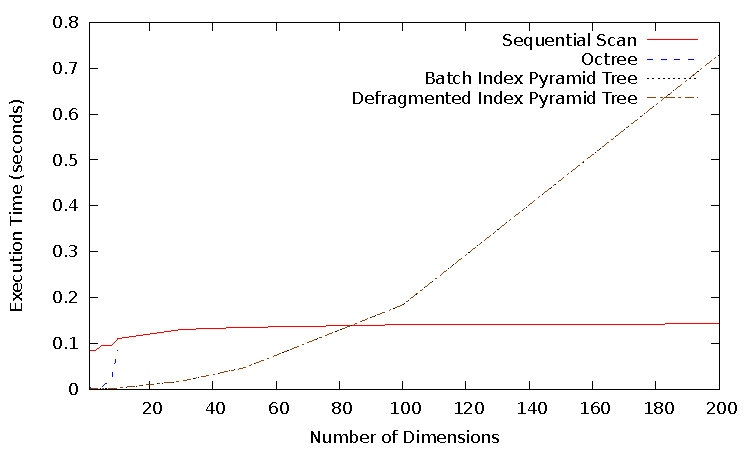
\includegraphics[scale=0.8]{figures/performance_analysis/iteration_1/all_pquery_randuniform.pdf}
	\caption{Point Query Performance on Randomly Generated Uniformly Distributed Datasets}
	\label{fig:perf-1-allpquery-d}
\end{figure}

\subsection{Profiling Results}

TODO: CPU and heap profiling

\subsection{Evaluation}

TODO: evaluate results in previous section

TODO state what was decided to do for next iteration (and why)
